\documentclass[11pt]{article}
\usepackage[a4paper,margin=1in]{geometry}
\usepackage{amsmath,amssymb,amsthm}
\usepackage{tikz}
\usepackage{xcolor}
\usepackage[hidelinks]{hyperref}
\hypersetup{pdftitle={Sixteen words},pdfauthor={Vamshi Jandhyala}}
\setlength{\parskip}{0.4em}
\setlength{\parindent}{0pt}

\newtheorem{theorem}{Theorem}
\newtheorem{corollary}{Corollary}
\newtheorem{lemma}{Lemma}
\newtheorem{proposition}{Proposition}
\theoremstyle{remark}
\newtheorem*{remark}{Remark}

\definecolor{inkblue}{RGB}{40,76,105}
\definecolor{softblue}{RGB}{226,235,243}
\definecolor{rust}{RGB}{153,70,45}

\title{Sixteen words cover all 15-bit strings}
\author{Vamshi Jandhyala}
\date{}

\begin{document}
\maketitle
\vspace{-2em}

\begin{abstract}
From every binary string of length $n=3k$ delete $k$ bits, choosing the deletions so that as few distinct
strings of length $2k$ remain as possible. The least number $H(3k,k)$ grows like $\alpha^{3k}$. We give sixteen
strings of length $10$ such that every string of length $15$ contains one of them as a subsequence, so
$H(15,5)\le16$, improving the bound $17$ from 2013, and hence $\alpha\le16^{1/15}<1.2031$. The set is closed
under complement and reversal, and among such sets sixteen is optimal; that claim is a computer result, certified
by a checked unsatisfiability proof. The argument from the cover to the bound on $\alpha$ is checked in the Lean
proof assistant.
\end{abstract}

\section{The question}

Take all $2^n$ binary strings of length $n$, with $n=3k$, and from each delete exactly $k$ bits. The deletions
may be chosen separately for each string, and the aim is to leave as few different strings of length $2k$ as
possible. How few? The question was asked on MathOverflow in 2013~\cite{MO}. Stop and try $n=3$ before reading
on: every string of length 3 has two equal bits, so deleting the odd bit leaves $00$ or $11$, and two strings
suffice.

Write $H(n,b)$ for the least number of strings of length $n-b$ that are left when $b$ bits are deleted from
each string of length $n$. Equivalently, it is the size of the smallest set $S$ of strings of length $n-b$ such
that every string of length $n$ contains a member of $S$ as a subsequence; we say $S$ \emph{covers} length $n$.
In coding-theory terms $S$ is a binary insertion covering code~\cite{LRSY21,XSG26}; those papers bound such
codes for a fixed number of insertions, while here the number grows with the length.

The 2013 discussion found the following. Splitting a string into blocks and treating each block separately
gives $H(n_1+n_2,b_1+b_2)\le H(n_1,b_1)\,H(n_2,b_2)$, so by Fekete's lemma
$\alpha=\lim H(3k,k)^{1/(3k)}$ exists and equals the infimum (Meyerowitz, Sawin~\cite{MO}). Each small cover gives an upper bound:
$H(3,1)=2$ gives $2^{1/3}\approx1.260$, Goucher's six words for $n=9$ give $6^{1/9}\approx1.220$, Meyerowitz's
ten words for $n=12$ give $10^{1/12}\approx1.212$, and a seventeen-word cover for $n=15$, recorded in the
question, gives $17^{1/15}\approx1.208$. Counting, as McKay and Yury showed, gives
$\alpha\ge2^{5/3}/3\approx1.058$~\cite{MO}. The question also records $12\le H(15,5)$.

\begin{theorem}\label{thm:main}
The sixteen strings of length 10
\[
\begin{array}{llll}
0000000000 & 0000000011 & 0000111110 & 0011001100\\
0011111111 & 0110000110 & 0110101001 & 0111110000\\
1000001111 & 1001010110 & 1001111001 & 1100000000\\
1100110011 & 1111000001 & 1111111100 & 1111111111
\end{array}
\]
cover length 15: every binary string of length 15 contains one of them as a subsequence. No proper subset
does. Hence $H(15,5)\le16$.
\end{theorem}

\begin{corollary}\label{cor:rate}
$\alpha\le16^{1/15}<1.2031$, against $17^{1/15}>1.2078$ before.
\end{corollary}

\begin{figure}[ht]
\centering
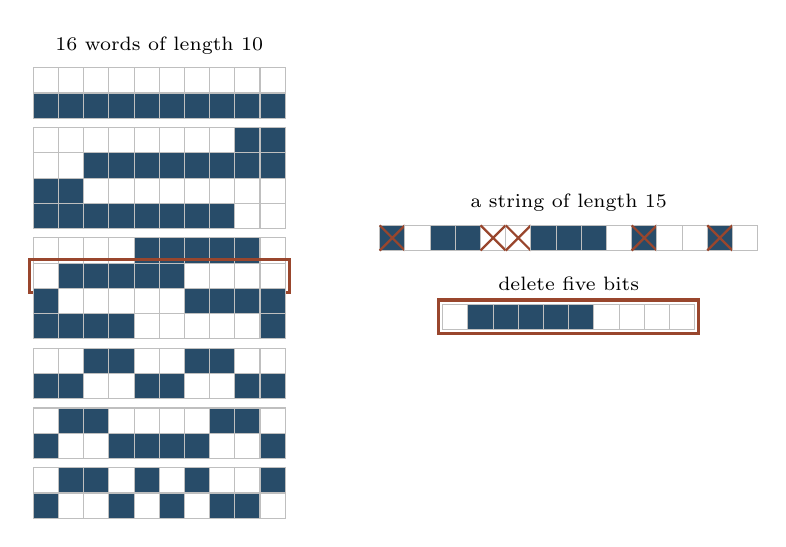
\begin{tikzpicture}[x=1cm,y=1cm]
  \filldraw[fill=white,draw=gray!50] (0.00,-0.00) rectangle ++(0.32,-0.32);
  \filldraw[fill=white,draw=gray!50] (0.32,-0.00) rectangle ++(0.32,-0.32);
  \filldraw[fill=white,draw=gray!50] (0.64,-0.00) rectangle ++(0.32,-0.32);
  \filldraw[fill=white,draw=gray!50] (0.96,-0.00) rectangle ++(0.32,-0.32);
  \filldraw[fill=white,draw=gray!50] (1.28,-0.00) rectangle ++(0.32,-0.32);
  \filldraw[fill=white,draw=gray!50] (1.60,-0.00) rectangle ++(0.32,-0.32);
  \filldraw[fill=white,draw=gray!50] (1.92,-0.00) rectangle ++(0.32,-0.32);
  \filldraw[fill=white,draw=gray!50] (2.24,-0.00) rectangle ++(0.32,-0.32);
  \filldraw[fill=white,draw=gray!50] (2.56,-0.00) rectangle ++(0.32,-0.32);
  \filldraw[fill=white,draw=gray!50] (2.88,-0.00) rectangle ++(0.32,-0.32);
  \filldraw[fill=inkblue,draw=gray!50] (0.00,-0.32) rectangle ++(0.32,-0.32);
  \filldraw[fill=inkblue,draw=gray!50] (0.32,-0.32) rectangle ++(0.32,-0.32);
  \filldraw[fill=inkblue,draw=gray!50] (0.64,-0.32) rectangle ++(0.32,-0.32);
  \filldraw[fill=inkblue,draw=gray!50] (0.96,-0.32) rectangle ++(0.32,-0.32);
  \filldraw[fill=inkblue,draw=gray!50] (1.28,-0.32) rectangle ++(0.32,-0.32);
  \filldraw[fill=inkblue,draw=gray!50] (1.60,-0.32) rectangle ++(0.32,-0.32);
  \filldraw[fill=inkblue,draw=gray!50] (1.92,-0.32) rectangle ++(0.32,-0.32);
  \filldraw[fill=inkblue,draw=gray!50] (2.24,-0.32) rectangle ++(0.32,-0.32);
  \filldraw[fill=inkblue,draw=gray!50] (2.56,-0.32) rectangle ++(0.32,-0.32);
  \filldraw[fill=inkblue,draw=gray!50] (2.88,-0.32) rectangle ++(0.32,-0.32);
  \filldraw[fill=white,draw=gray!50] (0.00,-0.76) rectangle ++(0.32,-0.32);
  \filldraw[fill=white,draw=gray!50] (0.32,-0.76) rectangle ++(0.32,-0.32);
  \filldraw[fill=white,draw=gray!50] (0.64,-0.76) rectangle ++(0.32,-0.32);
  \filldraw[fill=white,draw=gray!50] (0.96,-0.76) rectangle ++(0.32,-0.32);
  \filldraw[fill=white,draw=gray!50] (1.28,-0.76) rectangle ++(0.32,-0.32);
  \filldraw[fill=white,draw=gray!50] (1.60,-0.76) rectangle ++(0.32,-0.32);
  \filldraw[fill=white,draw=gray!50] (1.92,-0.76) rectangle ++(0.32,-0.32);
  \filldraw[fill=white,draw=gray!50] (2.24,-0.76) rectangle ++(0.32,-0.32);
  \filldraw[fill=inkblue,draw=gray!50] (2.56,-0.76) rectangle ++(0.32,-0.32);
  \filldraw[fill=inkblue,draw=gray!50] (2.88,-0.76) rectangle ++(0.32,-0.32);
  \filldraw[fill=white,draw=gray!50] (0.00,-1.08) rectangle ++(0.32,-0.32);
  \filldraw[fill=white,draw=gray!50] (0.32,-1.08) rectangle ++(0.32,-0.32);
  \filldraw[fill=inkblue,draw=gray!50] (0.64,-1.08) rectangle ++(0.32,-0.32);
  \filldraw[fill=inkblue,draw=gray!50] (0.96,-1.08) rectangle ++(0.32,-0.32);
  \filldraw[fill=inkblue,draw=gray!50] (1.28,-1.08) rectangle ++(0.32,-0.32);
  \filldraw[fill=inkblue,draw=gray!50] (1.60,-1.08) rectangle ++(0.32,-0.32);
  \filldraw[fill=inkblue,draw=gray!50] (1.92,-1.08) rectangle ++(0.32,-0.32);
  \filldraw[fill=inkblue,draw=gray!50] (2.24,-1.08) rectangle ++(0.32,-0.32);
  \filldraw[fill=inkblue,draw=gray!50] (2.56,-1.08) rectangle ++(0.32,-0.32);
  \filldraw[fill=inkblue,draw=gray!50] (2.88,-1.08) rectangle ++(0.32,-0.32);
  \filldraw[fill=inkblue,draw=gray!50] (0.00,-1.40) rectangle ++(0.32,-0.32);
  \filldraw[fill=inkblue,draw=gray!50] (0.32,-1.40) rectangle ++(0.32,-0.32);
  \filldraw[fill=white,draw=gray!50] (0.64,-1.40) rectangle ++(0.32,-0.32);
  \filldraw[fill=white,draw=gray!50] (0.96,-1.40) rectangle ++(0.32,-0.32);
  \filldraw[fill=white,draw=gray!50] (1.28,-1.40) rectangle ++(0.32,-0.32);
  \filldraw[fill=white,draw=gray!50] (1.60,-1.40) rectangle ++(0.32,-0.32);
  \filldraw[fill=white,draw=gray!50] (1.92,-1.40) rectangle ++(0.32,-0.32);
  \filldraw[fill=white,draw=gray!50] (2.24,-1.40) rectangle ++(0.32,-0.32);
  \filldraw[fill=white,draw=gray!50] (2.56,-1.40) rectangle ++(0.32,-0.32);
  \filldraw[fill=white,draw=gray!50] (2.88,-1.40) rectangle ++(0.32,-0.32);
  \filldraw[fill=inkblue,draw=gray!50] (0.00,-1.72) rectangle ++(0.32,-0.32);
  \filldraw[fill=inkblue,draw=gray!50] (0.32,-1.72) rectangle ++(0.32,-0.32);
  \filldraw[fill=inkblue,draw=gray!50] (0.64,-1.72) rectangle ++(0.32,-0.32);
  \filldraw[fill=inkblue,draw=gray!50] (0.96,-1.72) rectangle ++(0.32,-0.32);
  \filldraw[fill=inkblue,draw=gray!50] (1.28,-1.72) rectangle ++(0.32,-0.32);
  \filldraw[fill=inkblue,draw=gray!50] (1.60,-1.72) rectangle ++(0.32,-0.32);
  \filldraw[fill=inkblue,draw=gray!50] (1.92,-1.72) rectangle ++(0.32,-0.32);
  \filldraw[fill=inkblue,draw=gray!50] (2.24,-1.72) rectangle ++(0.32,-0.32);
  \filldraw[fill=white,draw=gray!50] (2.56,-1.72) rectangle ++(0.32,-0.32);
  \filldraw[fill=white,draw=gray!50] (2.88,-1.72) rectangle ++(0.32,-0.32);
  \filldraw[fill=white,draw=gray!50] (0.00,-2.16) rectangle ++(0.32,-0.32);
  \filldraw[fill=white,draw=gray!50] (0.32,-2.16) rectangle ++(0.32,-0.32);
  \filldraw[fill=white,draw=gray!50] (0.64,-2.16) rectangle ++(0.32,-0.32);
  \filldraw[fill=white,draw=gray!50] (0.96,-2.16) rectangle ++(0.32,-0.32);
  \filldraw[fill=inkblue,draw=gray!50] (1.28,-2.16) rectangle ++(0.32,-0.32);
  \filldraw[fill=inkblue,draw=gray!50] (1.60,-2.16) rectangle ++(0.32,-0.32);
  \filldraw[fill=inkblue,draw=gray!50] (1.92,-2.16) rectangle ++(0.32,-0.32);
  \filldraw[fill=inkblue,draw=gray!50] (2.24,-2.16) rectangle ++(0.32,-0.32);
  \filldraw[fill=inkblue,draw=gray!50] (2.56,-2.16) rectangle ++(0.32,-0.32);
  \filldraw[fill=white,draw=gray!50] (2.88,-2.16) rectangle ++(0.32,-0.32);
  \filldraw[fill=white,draw=gray!50] (0.00,-2.48) rectangle ++(0.32,-0.32);
  \filldraw[fill=inkblue,draw=gray!50] (0.32,-2.48) rectangle ++(0.32,-0.32);
  \filldraw[fill=inkblue,draw=gray!50] (0.64,-2.48) rectangle ++(0.32,-0.32);
  \filldraw[fill=inkblue,draw=gray!50] (0.96,-2.48) rectangle ++(0.32,-0.32);
  \filldraw[fill=inkblue,draw=gray!50] (1.28,-2.48) rectangle ++(0.32,-0.32);
  \filldraw[fill=inkblue,draw=gray!50] (1.60,-2.48) rectangle ++(0.32,-0.32);
  \filldraw[fill=white,draw=gray!50] (1.92,-2.48) rectangle ++(0.32,-0.32);
  \filldraw[fill=white,draw=gray!50] (2.24,-2.48) rectangle ++(0.32,-0.32);
  \filldraw[fill=white,draw=gray!50] (2.56,-2.48) rectangle ++(0.32,-0.32);
  \filldraw[fill=white,draw=gray!50] (2.88,-2.48) rectangle ++(0.32,-0.32);
  \draw[rust,very thick] (-0.05,-2.43) rectangle (3.25,-2.85);
  \filldraw[fill=inkblue,draw=gray!50] (0.00,-2.80) rectangle ++(0.32,-0.32);
  \filldraw[fill=white,draw=gray!50] (0.32,-2.80) rectangle ++(0.32,-0.32);
  \filldraw[fill=white,draw=gray!50] (0.64,-2.80) rectangle ++(0.32,-0.32);
  \filldraw[fill=white,draw=gray!50] (0.96,-2.80) rectangle ++(0.32,-0.32);
  \filldraw[fill=white,draw=gray!50] (1.28,-2.80) rectangle ++(0.32,-0.32);
  \filldraw[fill=white,draw=gray!50] (1.60,-2.80) rectangle ++(0.32,-0.32);
  \filldraw[fill=inkblue,draw=gray!50] (1.92,-2.80) rectangle ++(0.32,-0.32);
  \filldraw[fill=inkblue,draw=gray!50] (2.24,-2.80) rectangle ++(0.32,-0.32);
  \filldraw[fill=inkblue,draw=gray!50] (2.56,-2.80) rectangle ++(0.32,-0.32);
  \filldraw[fill=inkblue,draw=gray!50] (2.88,-2.80) rectangle ++(0.32,-0.32);
  \filldraw[fill=inkblue,draw=gray!50] (0.00,-3.12) rectangle ++(0.32,-0.32);
  \filldraw[fill=inkblue,draw=gray!50] (0.32,-3.12) rectangle ++(0.32,-0.32);
  \filldraw[fill=inkblue,draw=gray!50] (0.64,-3.12) rectangle ++(0.32,-0.32);
  \filldraw[fill=inkblue,draw=gray!50] (0.96,-3.12) rectangle ++(0.32,-0.32);
  \filldraw[fill=white,draw=gray!50] (1.28,-3.12) rectangle ++(0.32,-0.32);
  \filldraw[fill=white,draw=gray!50] (1.60,-3.12) rectangle ++(0.32,-0.32);
  \filldraw[fill=white,draw=gray!50] (1.92,-3.12) rectangle ++(0.32,-0.32);
  \filldraw[fill=white,draw=gray!50] (2.24,-3.12) rectangle ++(0.32,-0.32);
  \filldraw[fill=white,draw=gray!50] (2.56,-3.12) rectangle ++(0.32,-0.32);
  \filldraw[fill=inkblue,draw=gray!50] (2.88,-3.12) rectangle ++(0.32,-0.32);
  \filldraw[fill=white,draw=gray!50] (0.00,-3.56) rectangle ++(0.32,-0.32);
  \filldraw[fill=white,draw=gray!50] (0.32,-3.56) rectangle ++(0.32,-0.32);
  \filldraw[fill=inkblue,draw=gray!50] (0.64,-3.56) rectangle ++(0.32,-0.32);
  \filldraw[fill=inkblue,draw=gray!50] (0.96,-3.56) rectangle ++(0.32,-0.32);
  \filldraw[fill=white,draw=gray!50] (1.28,-3.56) rectangle ++(0.32,-0.32);
  \filldraw[fill=white,draw=gray!50] (1.60,-3.56) rectangle ++(0.32,-0.32);
  \filldraw[fill=inkblue,draw=gray!50] (1.92,-3.56) rectangle ++(0.32,-0.32);
  \filldraw[fill=inkblue,draw=gray!50] (2.24,-3.56) rectangle ++(0.32,-0.32);
  \filldraw[fill=white,draw=gray!50] (2.56,-3.56) rectangle ++(0.32,-0.32);
  \filldraw[fill=white,draw=gray!50] (2.88,-3.56) rectangle ++(0.32,-0.32);
  \filldraw[fill=inkblue,draw=gray!50] (0.00,-3.88) rectangle ++(0.32,-0.32);
  \filldraw[fill=inkblue,draw=gray!50] (0.32,-3.88) rectangle ++(0.32,-0.32);
  \filldraw[fill=white,draw=gray!50] (0.64,-3.88) rectangle ++(0.32,-0.32);
  \filldraw[fill=white,draw=gray!50] (0.96,-3.88) rectangle ++(0.32,-0.32);
  \filldraw[fill=inkblue,draw=gray!50] (1.28,-3.88) rectangle ++(0.32,-0.32);
  \filldraw[fill=inkblue,draw=gray!50] (1.60,-3.88) rectangle ++(0.32,-0.32);
  \filldraw[fill=white,draw=gray!50] (1.92,-3.88) rectangle ++(0.32,-0.32);
  \filldraw[fill=white,draw=gray!50] (2.24,-3.88) rectangle ++(0.32,-0.32);
  \filldraw[fill=inkblue,draw=gray!50] (2.56,-3.88) rectangle ++(0.32,-0.32);
  \filldraw[fill=inkblue,draw=gray!50] (2.88,-3.88) rectangle ++(0.32,-0.32);
  \filldraw[fill=white,draw=gray!50] (0.00,-4.32) rectangle ++(0.32,-0.32);
  \filldraw[fill=inkblue,draw=gray!50] (0.32,-4.32) rectangle ++(0.32,-0.32);
  \filldraw[fill=inkblue,draw=gray!50] (0.64,-4.32) rectangle ++(0.32,-0.32);
  \filldraw[fill=white,draw=gray!50] (0.96,-4.32) rectangle ++(0.32,-0.32);
  \filldraw[fill=white,draw=gray!50] (1.28,-4.32) rectangle ++(0.32,-0.32);
  \filldraw[fill=white,draw=gray!50] (1.60,-4.32) rectangle ++(0.32,-0.32);
  \filldraw[fill=white,draw=gray!50] (1.92,-4.32) rectangle ++(0.32,-0.32);
  \filldraw[fill=inkblue,draw=gray!50] (2.24,-4.32) rectangle ++(0.32,-0.32);
  \filldraw[fill=inkblue,draw=gray!50] (2.56,-4.32) rectangle ++(0.32,-0.32);
  \filldraw[fill=white,draw=gray!50] (2.88,-4.32) rectangle ++(0.32,-0.32);
  \filldraw[fill=inkblue,draw=gray!50] (0.00,-4.64) rectangle ++(0.32,-0.32);
  \filldraw[fill=white,draw=gray!50] (0.32,-4.64) rectangle ++(0.32,-0.32);
  \filldraw[fill=white,draw=gray!50] (0.64,-4.64) rectangle ++(0.32,-0.32);
  \filldraw[fill=inkblue,draw=gray!50] (0.96,-4.64) rectangle ++(0.32,-0.32);
  \filldraw[fill=inkblue,draw=gray!50] (1.28,-4.64) rectangle ++(0.32,-0.32);
  \filldraw[fill=inkblue,draw=gray!50] (1.60,-4.64) rectangle ++(0.32,-0.32);
  \filldraw[fill=inkblue,draw=gray!50] (1.92,-4.64) rectangle ++(0.32,-0.32);
  \filldraw[fill=white,draw=gray!50] (2.24,-4.64) rectangle ++(0.32,-0.32);
  \filldraw[fill=white,draw=gray!50] (2.56,-4.64) rectangle ++(0.32,-0.32);
  \filldraw[fill=inkblue,draw=gray!50] (2.88,-4.64) rectangle ++(0.32,-0.32);
  \filldraw[fill=white,draw=gray!50] (0.00,-5.08) rectangle ++(0.32,-0.32);
  \filldraw[fill=inkblue,draw=gray!50] (0.32,-5.08) rectangle ++(0.32,-0.32);
  \filldraw[fill=inkblue,draw=gray!50] (0.64,-5.08) rectangle ++(0.32,-0.32);
  \filldraw[fill=white,draw=gray!50] (0.96,-5.08) rectangle ++(0.32,-0.32);
  \filldraw[fill=inkblue,draw=gray!50] (1.28,-5.08) rectangle ++(0.32,-0.32);
  \filldraw[fill=white,draw=gray!50] (1.60,-5.08) rectangle ++(0.32,-0.32);
  \filldraw[fill=inkblue,draw=gray!50] (1.92,-5.08) rectangle ++(0.32,-0.32);
  \filldraw[fill=white,draw=gray!50] (2.24,-5.08) rectangle ++(0.32,-0.32);
  \filldraw[fill=white,draw=gray!50] (2.56,-5.08) rectangle ++(0.32,-0.32);
  \filldraw[fill=inkblue,draw=gray!50] (2.88,-5.08) rectangle ++(0.32,-0.32);
  \filldraw[fill=inkblue,draw=gray!50] (0.00,-5.40) rectangle ++(0.32,-0.32);
  \filldraw[fill=white,draw=gray!50] (0.32,-5.40) rectangle ++(0.32,-0.32);
  \filldraw[fill=white,draw=gray!50] (0.64,-5.40) rectangle ++(0.32,-0.32);
  \filldraw[fill=inkblue,draw=gray!50] (0.96,-5.40) rectangle ++(0.32,-0.32);
  \filldraw[fill=white,draw=gray!50] (1.28,-5.40) rectangle ++(0.32,-0.32);
  \filldraw[fill=inkblue,draw=gray!50] (1.60,-5.40) rectangle ++(0.32,-0.32);
  \filldraw[fill=white,draw=gray!50] (1.92,-5.40) rectangle ++(0.32,-0.32);
  \filldraw[fill=inkblue,draw=gray!50] (2.24,-5.40) rectangle ++(0.32,-0.32);
  \filldraw[fill=inkblue,draw=gray!50] (2.56,-5.40) rectangle ++(0.32,-0.32);
  \filldraw[fill=white,draw=gray!50] (2.88,-5.40) rectangle ++(0.32,-0.32);
  \node[font=\scriptsize,anchor=south] at (1.60,0.05) {16 words of length 10};
  \node[font=\scriptsize,anchor=south] at (6.80,-1.95) {a string of length 15};
  \filldraw[fill=inkblue,draw=gray!50] (4.40,-2.00) rectangle ++(0.32,-0.32);
  \draw[rust,thick] (4.40,-2.00) -- ++(0.32,-0.32) (4.40,-2.32) -- ++(0.32,0.32);
  \filldraw[fill=white,draw=gray!50] (4.72,-2.00) rectangle ++(0.32,-0.32);
  \filldraw[fill=inkblue,draw=gray!50] (5.04,-2.00) rectangle ++(0.32,-0.32);
  \filldraw[fill=inkblue,draw=gray!50] (5.36,-2.00) rectangle ++(0.32,-0.32);
  \filldraw[fill=white,draw=gray!50] (5.68,-2.00) rectangle ++(0.32,-0.32);
  \draw[rust,thick] (5.68,-2.00) -- ++(0.32,-0.32) (5.68,-2.32) -- ++(0.32,0.32);
  \filldraw[fill=white,draw=gray!50] (6.00,-2.00) rectangle ++(0.32,-0.32);
  \draw[rust,thick] (6.00,-2.00) -- ++(0.32,-0.32) (6.00,-2.32) -- ++(0.32,0.32);
  \filldraw[fill=inkblue,draw=gray!50] (6.32,-2.00) rectangle ++(0.32,-0.32);
  \filldraw[fill=inkblue,draw=gray!50] (6.64,-2.00) rectangle ++(0.32,-0.32);
  \filldraw[fill=inkblue,draw=gray!50] (6.96,-2.00) rectangle ++(0.32,-0.32);
  \filldraw[fill=white,draw=gray!50] (7.28,-2.00) rectangle ++(0.32,-0.32);
  \filldraw[fill=inkblue,draw=gray!50] (7.60,-2.00) rectangle ++(0.32,-0.32);
  \draw[rust,thick] (7.60,-2.00) -- ++(0.32,-0.32) (7.60,-2.32) -- ++(0.32,0.32);
  \filldraw[fill=white,draw=gray!50] (7.92,-2.00) rectangle ++(0.32,-0.32);
  \filldraw[fill=white,draw=gray!50] (8.24,-2.00) rectangle ++(0.32,-0.32);
  \filldraw[fill=inkblue,draw=gray!50] (8.56,-2.00) rectangle ++(0.32,-0.32);
  \draw[rust,thick] (8.56,-2.00) -- ++(0.32,-0.32) (8.56,-2.32) -- ++(0.32,0.32);
  \filldraw[fill=white,draw=gray!50] (8.88,-2.00) rectangle ++(0.32,-0.32);
  \node[font=\scriptsize,anchor=south] at (6.80,-2.95) {delete five bits};
  \filldraw[fill=white,draw=gray!50] (5.20,-3.00) rectangle ++(0.32,-0.32);
  \filldraw[fill=inkblue,draw=gray!50] (5.52,-3.00) rectangle ++(0.32,-0.32);
  \filldraw[fill=inkblue,draw=gray!50] (5.84,-3.00) rectangle ++(0.32,-0.32);
  \filldraw[fill=inkblue,draw=gray!50] (6.16,-3.00) rectangle ++(0.32,-0.32);
  \filldraw[fill=inkblue,draw=gray!50] (6.48,-3.00) rectangle ++(0.32,-0.32);
  \filldraw[fill=inkblue,draw=gray!50] (6.80,-3.00) rectangle ++(0.32,-0.32);
  \filldraw[fill=white,draw=gray!50] (7.12,-3.00) rectangle ++(0.32,-0.32);
  \filldraw[fill=white,draw=gray!50] (7.44,-3.00) rectangle ++(0.32,-0.32);
  \filldraw[fill=white,draw=gray!50] (7.76,-3.00) rectangle ++(0.32,-0.32);
  \filldraw[fill=white,draw=gray!50] (8.08,-3.00) rectangle ++(0.32,-0.32);
  \draw[rust,very thick] (5.15,-2.95) rectangle (8.45,-3.37);
\end{tikzpicture}

\caption{Left: the sixteen words, one per row (dark cells are $1$), grouped into the six orbits of complement
and reversal. Right: a string of length 15; deleting the five crossed bits leaves the outlined word.}
\label{fig:cover}
\end{figure}

\begin{proposition}\label{prop:sym}
No set of fifteen or fewer strings of length 10 that is closed under complement and under reversal covers
length 15.
\end{proposition}

Proposition~\ref{prop:sym} is a computer result, so it is worth saying how it is checked. The search space
is described in Section~\ref{sec:search}; the infeasibility was found by one solver, confirmed by a second with
a different encoding, and the second solver's proof of unsatisfiability was checked by an independent proof
checker. Whether a cover of size 15 exists without the symmetry is open. A 100-second unrestricted search
neither found one nor ruled it out.

\section{From a cover to the growth rate}

\begin{lemma}[blocks]\label{lem:blocks}
If $S$ covers length $n_1$ with strings of length $m_1$ and $T$ covers length $n_2$ with strings of length
$m_2$, then the concatenations $\{st:s\in S,\ t\in T\}$ cover length $n_1+n_2$ with strings of length
$m_1+m_2$, and there are at most $|S|\,|T|$ of them.
\end{lemma}

\begin{proof}
Split a string of length $n_1+n_2$ into its first $n_1$ bits and the rest. The first part contains some $s\in S$
as a subsequence and the second some $t\in T$, so the whole contains $st$.
\end{proof}

So $H$ is submultiplicative, $\log H(3k,k)$ is subadditive in $k$, and Fekete's lemma gives the limit
$\alpha$ as an infimum. In particular $\alpha\le H(15,5)^{1/15}\le16^{1/15}$, which proves
Corollary~\ref{cor:rate}. Concretely, the $m$-fold concatenations of the sixteen words cover length $15m$ with
$16^m$ strings.

\section{How the cover was found}\label{sec:search}

Covering length 15 with strings of length 10 is a set-cover problem with $2^{10}=1024$ candidate strings and
$2^{15}=32768$ strings to cover. Meyerowitz suggested in the 2013 thread looking for covers closed under
complement and reversal~\cite{MO}. Both maps preserve the subsequence relation (applied to both strings), so a
union of orbits covers everything as soon as it covers one string from each orbit of length-15 strings. The
1024 strings fall into orbits of size 2 or 4, and one Boolean variable per orbit gives an exact model: one
clause per string of length 15 (or per orbit of them), listing the orbits with a member that is a subsequence of it, and a weighted
bound on the total size.

An exact solver (CP-SAT) finds a symmetric cover of size 16 and proves that none of size 15 exists, in a few
seconds on one core. The recheck builds its own clauses and its own cardinality encoding, solves them with
a different solver (Glucose), and writes a proof of unsatisfiability for size 15 that the independent checker
drat-trim verifies. The cover in Theorem~\ref{thm:main} is then checked by itself: a direct test of all $2^{15}$
strings, in two programs that share no code. Each of the sixteen words is needed: removing any one leaves some
string of length 15 uncovered.

\begin{remark}
To beat $16^{1/15}$ with the next length, $n=18$, needs a cover by at most 27 strings of length 12. An
eight-minute symmetric search found nothing below 30; that proves nothing either way. The exact value of
$\alpha$, which lies between $1.058$ and $1.2031$, is open, and so is $H(15,5)$, which lies between 12 and
16.
\end{remark}

\paragraph{Verification.} Lemma~\ref{lem:blocks}, the submultiplicativity of $H$, the existence of $\alpha$
by Fekete's lemma (Mathlib's \texttt{Subadditive.tendsto\_lim}), the bound $\alpha\le16^{1/15}$ from a
sixteen-word cover, and the numerical bounds on $16^{1/15}$ and $17^{1/15}$ are checked in Lean~4 with
Mathlib~\cite{mathlib}, using only the standard axioms. The cover itself and Proposition~\ref{prop:sym} are
finite computations, checked as described in Section~\ref{sec:search} and not in Lean. Everything is at
\url{https://github.com/jvvk/mathematics/tree/main/sixteen-words}.

\paragraph{Acknowledgements.} The question was asked by user45564 on MathOverflow; the earlier bounds are
due to the people named above, in that thread. Anthropic's Claude (Opus~5.5) was used to set up the searches,
write the Lean formalisation and the programs, and draft this text. The author takes responsibility for the
content.

\begin{thebibliography}{9}
\bibitem{LRSY21} A.~Lenz, C.~Rashtchian, P.~H.~Siegel and E.~Yaakobi, Covering codes using insertions or
deletions, \emph{IEEE Trans. Inform. Theory} \textbf{67} (2021) 3376--3388,
\href{https://doi.org/10.1109/TIT.2020.2985691}{doi:10.1109/TIT.2020.2985691}.
\bibitem{MO} user45564, Puzzle on deleting $k$ bits from binary vectors of length $3k$, MathOverflow
question 142857 (22 September 2013), with answers by A.~P.~Goucher, A.~Meyerowitz, B.~McKay, Yury,
W.~Sawin and others, \url{https://mathoverflow.net/q/142857}, accessed 10 October 2026.
\bibitem{XSG26} C.~Xie, Y.~Sun and G.~Ge, New bounds for covering codes under insertions or deletions,
arXiv:2606.15379 (2026).
\bibitem{mathlib} The mathlib Community, The Lean mathematical library, in \emph{Proceedings of the 9th ACM
SIGPLAN International Conference on Certified Programs and Proofs (CPP 2020)}, 367--381,
\href{https://doi.org/10.1145/3372885.3373824}{doi:10.1145/3372885.3373824}.
\end{thebibliography}

\bigskip
\noindent Vamshi Jandhyala, London, UK.

\end{document}
